\documentclass{report}
\usepackage{background}
\usetikzlibrary{calc}
\usepackage{ifthen}
\usepackage{lipsum}
\usepackage[a4paper, left=35mm,top=7mm,bottom=25mm]{geometry}
\pagestyle{plain} %Allows using symbols 

\usepackage[fleqn]{amsmath} %% flegn = align left, %% math equation package
\usepackage{caption} %% allows caption
\usepackage{wrapfig} %% allows wrapping of text around figures


% background common settings
\SetBgScale{1}
\SetBgAngle{0}
\SetBgOpacity{1}
\SetBgContents{}

% auxiliary counter
\newcounter{chapshift}
\addtocounter{chapshift}{-1}

% the list of colors to be used (add more if needed)
\newcommand\BoxColor{%
  \ifcase\thechapshift black!100 \or black!80\or black!60\or black!40\else black!30\fi}

% the main command; the mandatory argument sets the color of the vertical box
\makeatletter
\newcommand\ChapFrame{%
\AddEverypageHook{%
\ifthenelse{\isodd{\thepage}}
{\SetBgContents{%
  
\begin{tikzpicture}[overlay,remember picture]
  \node[fill=\BoxColor,inner sep=0pt,rectangle,text width=1.5cm,
    text height=1.5cm,align=center,anchor=north east] 
  at ($ (current page.north east) + (-0cm,-2*\thechapshift cm) $) 
  {{\hspace*{0.5cm}\parbox[c][2.5cm][c]{1cm}{%
    \Huge\raggedright\textcolor{white}{\scshape\leftmark}}}};
  \end{tikzpicture}}%
}
{\SetBgContents{%
  
\begin{tikzpicture}[overlay,remember picture]
  \node[fill=\BoxColor,inner sep=0pt,rectangle,text width=1.5cm,
    text height=1.5cm,align=center,anchor=north west] 
  at ($ (current page.north west) + (-0cm,-2*\thechapshift cm) $) 
  {{\hspace*{0.5cm}\parbox[c][2.5cm][c]{1cm}{%
    \Huge\raggedright\textcolor{white}{\scshape\leftmark}}}};
  \end{tikzpicture}}
}
\bg@material}%
  \stepcounter{chapshift}
}
\makeatother

% redefinition of \chaptermark to contain only the title
\renewcommand\chaptermark[1]{\markboth{\thechapter}{}} 
\usepackage{titlesec}
\titleformat{\chapter}{\huge\bfseries}{\thechapter. }{0pt}{\huge \bfseries}

% Bibliography
\usepackage{natbib} 
\setcitestyle{authoryear,open={(},close={)}} 
\bibliographystyle{chicagoa}

\title{Jenny trying to understand TREMBLE}
\author{me}

% NEW COMMANDS FOR EQUATIONS 
\newcommand{\bmax}{B_{\rm max}}
\newcommand{\bpnd}{B\!P_{\rm ND}}
\newcommand{\bpndb}{B\!P_{\rm ND(b)}}
\newcommand{\bpndi}{B\!P_{\rm ND(i)}}
\newcommand{\cnd}{c_{\rm ND}(t)}
\newcommand{\ca}{c_{\rm a}(t)}
\newcommand{\cfp}{c_{\rm FP}(t)}
\newcommand{\cft}{c_{\rm FT}(t)}
\newcommand{\cnds}{C_{\rm ND}}
\newcommand{\cas}{C_{\rm a}}
\newcommand{\cfps}{C_{\rm FP}}
\newcommand{\cfts}{C_{\rm FT}}
\newcommand{\fp}{f_{\rm P}}
\newcommand{\kd}{K_{\rm D}}
\newcommand{\kone}{K_{\rm 1}}
\newcommand{\ktwo}{k'_{\rm 2}}
\newcommand{\vnd}{V_{\rm ND}}
\newcommand{\vndb}{V_{\rm ND(b)}}
\newcommand{\vndi}{V_{\rm ND(i)}}
\newcommand{\vd}{V_{\rm D}}
\newcommand{\vt}{V_{\rm T}}
\newcommand{\vtb}{V_{\rm T(b)}}
\newcommand{\vti}{V_{\rm T(i)}}
\newcommand{\cyoh}{$[^{11}{\rm C}]$yohimbine}
\newcommand{\cele}{$[^{11}{\rm C}]$}
\newcommand{\feigthteen}{$[^{18}{\rm F}]$}
\newcommand{\1}{$_1$}
\newcommand{\2}{$_2$}
\newcommand{\twoA}{$_{2 {\rm A}}$}
\newcommand{\alf}{$\alpha$}
\newcommand{\bet}{$\beta$}
\newcommand{\AR}{adrenoceptors}
\newcommand{\rsq}{$\rm R^2$}

%%%%%%%%%%%%%%%%%%%%%%%%%%%%%%%%%%%%%%%%%%%%%%%%%%%%%%%%%%%%%%%%%%%%%%%%%

\begin{document}

\maketitle

\chapter[My notes]{My Notes}
\ChapFrame 

\section*{I. Derivation of TREMBLE} 
	\begin{wrapfigure}{r}{.3\textwidth}
		\vspace{-15pt}
		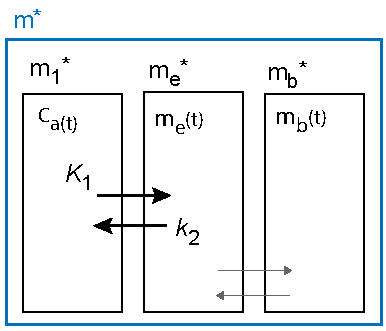
\includegraphics[width=1\linewidth]{exchangeable_compartment.pdf}
		\caption{}\label{fig1}
	\end{wrapfigure}

When there is more than three compartments, the number of parameters becomes so large that regression analysis fails to fit accurate estimates. 
The analysis can be simplified to describe tracer accumulation into a precursor compartment, which contains exchangeable ligands, $m_e^{*}$, which affects the transfer of ligand to the subsequent compartments \ref{dm1_dt}. The exchange of tracer from plasma to the precursor compartment can be described as follows,
	\begin{equation}\label{dm1_dt}
	\dfrac{dm_1(t)}{dt}=V_0\ \dfrac{d\ca}{dt},
	\end{equation}
	
\noindent
where $V_0$ is the volume of the vascular bed, $\ca$ is the time-variable concentration in plasma. The exchange of ligand from the precursor compartment to plasma is described as,

	\begin{equation}\label{dme_dt}
	\dfrac{dm_e(t)}{dt}=K_1\ \ca-k_2\ m_e(t),
	\end{equation}

\noindent
combination of eqs. \ref{dm1_dt} and \ref{dme_dt} yields the observed values, $m(t)$,
	\begin{equation}\label{dm_dt}
	\dfrac{dm(t)}{dt}=V_0\ \dfrac{d\ca}{dt} \ + \ \bigg( K_1\ \ca-k_2\ m_e(t) \bigg).
	\end{equation}
	
\noindent
By rearrangement of eq. \ref{dm_dt}, the content of ligand in the exchangeable compartment can also be expressed as, 

	\begin{align}\label{me(t)}
	\dfrac{dm_e(t)}{dt} = \dfrac{dm(t)}{dt} \ - \ V_0\ \dfrac{d\ca}{dt} = K_1\ \ca-k_2\ m_e(t)  \\ 
	\dfrac{1}{K_1}\bigg(\dfrac{dm(t)}{dt} \ - \ V_0\ \bigg)= \ca - \dfrac{k_2}{K_1} \ m_e(t) \\
	\dfrac{k_2}{K_1} m_e(t) = \ca - \dfrac{1}{K_1}\bigg(\dfrac{dm(t)}{dt} \ - \ V_0\ \bigg)	\\
	m_e(t)= V_e \Bigg[ 
	\ca - \dfrac{1}{K_1}\bigg(\dfrac{dm(t)}{dt} \ - \ V_0\ \bigg) 
	\Bigg],
	\end{align}
\noindent
where $V_e=K_1/k_2$ is the partition volume of exchangeable ligand (e.g. volume of distribution in cerebellum). 

	
	
	
\bibliography{JAP_references_2016_library}

\end{document}